%%%%%%%%%%%%%%%%% Format %%%%%%%%%%%%%%%%%%%%%%%%%

%\documentclass[preprint,12pt]{elsarticle}
%% Use the option review to obtain double line spacing
\documentclass[authoryear,preprint,review,12pt]{elsarticle}

%% Use the options 1p,twocolumn; 3p; 3p,twocolumn; 5p; or 5p,twocolumn
%% for a journal layout:
%\documentclass[final,1p,times]{elsarticle}
%%\documentclass[final,1p,times,twocolumn]{elsarticle}

%\documentclass[final,3p,times]{elsarticle}
%\documentclass[12pt,a4paper]{elsarticle}  % Assuming you're using elsarticle; adjust accordingly

%\documentclass[final,3p,times,twocolumn]{elsarticle}
%\documentclass[final,5p,times]{elsarticle}
%% \documentclass[final,5p,times,twocolumn]{elsarticle}

%% For including figures, graphicx.sty has been loaded in
%% elsarticle.cls. If you prefer to use the old commands
%% please give \usepackage{epsfig}

%% The amssymb package provides various useful mathematical symbols
\usepackage{amssymb}
%% The amsthm package provides extended theorem environments
\usepackage{amsthm}
\usepackage{makeidx}

%% The lineno packages adds line numbers. Start line numbering with
%% \begin{linenumbers}, end it with \end{linenumbers}. Or switch it on
%% for the whole article with \linenumbers.
%% \usepackage{lineno}

%\journal{CDT}

%%%%%%%%%%%%%%% Start of the report %%%%%%%%%%%%%%%%%%



\usepackage[utf8]{inputenc}
\usepackage[T1]{fontenc}
\usepackage{lmodern}
\usepackage{graphicx}
\usepackage{color}
\usepackage{hyperref}
\usepackage{amsmath}
\usepackage{amsfonts}
\usepackage{epstopdf}
\usepackage[table]{xcolor}
\usepackage[framed,numbered,autolinebreaks,useliterate]{mcode}
\usepackage{float}
\usepackage{matlab}
\usepackage{vmargin}
\usepackage{pdflscape}
\usepackage{chngcntr}
\usepackage{fancyhdr} % For customizing headers and footers
\usepackage{ragged2e}
\usepackage{titling}  % For custom title formatting
\usepackage{gensymb}
\usepackage{float}

\DeclareUnicodeCharacter{00B0}{\degree}
\counterwithin{figure}{section}
%\usepackage{natbib}
%\usepackage[numbers,sort&compress]{natbib}


\usepackage[backend=biber,style=numeric,sorting=none]{biblatex}
\addbibresource{references.bib} % Link to your .bib file

\usepackage{graphicx}
\usepackage{float}
\usepackage{placeins}


\makeindex

% Header and footer
\pagestyle{fancy}
\fancyhf{} 
\fancyhead[L]{\leftmark}
\fancyfoot[C]{\thepage} % Page number at the center of the footer

% Update the section name in the header
\renewcommand{\sectionmark}[1]{\markboth{\thesection\ #1}{}}

\usepackage{titlesec}

%\titleformat{\chapter}

% Remove section numbering
\titleformat{\section}
  {\Large\bfseries} % format
  {}                % label
  {0pt}             % sep
  {\huge}           % before-code

% Keep subsection numbering
\titleformat{\subsection}
  {\large\bfseries} % format
  {\thesubsection}  % label
  {1em}             % sep
  {}                % before-code


  
\begin{document}


%%%%%%%%%%%%%%%%%% START DOCUMENT %%%%%%%%%%%%%%%%%%
\pagenumbering{arabic}
\thispagestyle{empty} 

\centering
\vspace{4.4 in}

\fontsize{24}{24}\selectfont 

Add your title

\fontsize{14}{14}\selectfont 
\vspace{1.4 in}
A thesis submitted to the University of Manchester for the degree of Doctor of Philosophy in the Faculty of Science and Engineering.


\vspace{1.4 in}
\textbf{Add the year of submission}


\vspace{1 in}
\noindent
\textbf{Add your name}


\vspace{1.2 in}
\textbf{School of Natural Sciences, Department of Materials}

\clearpage


\begin{justify}

\tableofcontents

\clearpage

\listoffigures

\clearpage

\listoftables


\clearpage
\chapter{\fontsize{24pt}{20pt}\selectfont \textbf{Abstract}}
\thispagestyle{plain}
\vspace{0.1 in}
\noindent

Add your abstract

\clearpage
\thispagestyle{plain}
\chapter{\fontsize{24pt}{20pt}\selectfont \textbf{Declaration}}

\vspace{0.1 in}
\noindent

No portion of the work referred to in the thesis has been submitted in support of an application for another degree or qualification of this or any other university or other institute of learning.

\clearpage
\thispagestyle{plain}
\chapter{\fontsize{24pt}{20pt}\selectfont \textbf{Copyright statement}}

\vspace{0.1 in}
\noindent

\begin{itemize}
    \item The author of this thesis (including any appendices and/or schedules to this thesis) owns certain copyright or related rights in it (the “Copyright”) and they have given the University of Manchester certain rights to use such Copyright, including for administrative purposes.
    \item Copies of this thesis, either in full or in extracts and whether in hard or electronic copy, may be made only in accordance with the Copyright, Designs and Patents Act 1988 (as amended) and regulations issued under it or, where appropriate, in accordance with licensing agreements which the University has from time to time. This page must form part of any such copies made.
    \item The ownership of certain Copyright, patents, designs, trademarks and other intellectual property (the “Intellectual Property”) and any reproductions of copyright works in the thesis, for example graphs and tables (“Reproductions”), which may be described in this thesis, may not be owned by the author and may be owned by third parties. Such Intellectual Property and Reproductions cannot and must not be made available for use without the prior written permission of the owner(s) of the relevant Intellectual
    \item Further information on the conditions under which disclosure, publication and commercialisation of this thesis, the Copyright and any Intellectual Property and/or Reproductions described in it may take place is available in the \href{http://documents.manchester.ac.uk/DocuInfo.aspx?DocID=24420}{University IP Policy}, in any relevant Thesis restriction declarations deposited in the University Library, the  \href{http://www.library.manchester.ac.uk/about/regulations/}{University Library's regulations} and in the \href{https://documents.manchester.ac.uk/display.aspx?DocID=7420}{University's policy on Presentation of Theses}.
\end{itemize}





\clearpage
\thispagestyle{plain}

\vspace*{-2cm}  
\chapter{\fontsize{24pt}{20pt}\selectfont \textbf{Acknowledgements}}


\vspace{0.1 in}
\noindent

Add here your acknowledgements


\clearpage
\thispagestyle{plain}
(blank page)





\clearpage
\chapter{\fontsize{24pt}{20pt}\selectfont \textbf{Chapter 1}}
\section{Introduction}
\label{sec:introduction} 



\vspace{0.1 in}
\noindent

There is one .tex file per chapter and all of them are linked to Report.tex


\vspace{0.1 in}
\noindent
If you compile Report.tex, all the files linked to it will be displayed.

\vspace{0.1 in}
\noindent
You can add your references in the file references.bib

\vspace{0.1 in}
\noindent
The journals usually offer a direct download of a bib file with the reference already formatted. You can copy the text in that bib file and paste it in the references.bib file of this template.

\vspace{0.1 in}
\noindent
Cite your references \cite{UKGovernment} when needed. You can add more than one reference \cite{ZHENG201855, ZHENG201855, Das2010RecyclingVehicles}.

\vspace{0.1 in}
\noindent
The label at the beginning of each section allows you to cite this chapter in the following chapters


\vspace{0.1 in}
\noindent

\subsection{\textbf{Add subsections}}

\vspace{0.1 in}
\noindent

\subsubsection{\textbf{And subsubsections}}


\vspace{0.1 in}
\noindent

Use this structure to add bullet points:

\begin{itemize}

\item Objective 1

\item This is my objective 2

\item And my objective 3

\end{itemize}






\clearpage
\chapter{\fontsize{24pt}{20pt}\selectfont \textbf{Chapter 2}}
\section{Literature Review}
\label{sec:litreview}

You can mention previous chapters, like Chapter \ref{sec:introduction}, using the label that you have written before.

\subsection{\textbf{Add the title of your subsection here}}
\label{sec:labelname}

\vspace{0.1 in}
\noindent
You can also add labels to a subsection, like in \ref{sec:labelname}




\vspace{0.1 in}
\noindent


Let's add one equation that you can cite in your text \ref{eq:name_of_your_equation}

\vspace{0.1 in}
\noindent

\begin{equation}
\label{eq:name_of_your_equation}
y = mx + n
\end{equation}


\vspace{0.1 in}
\noindent

Let's add a table that you can reference in the text too, Table \ref{table:myparameters}. I prefer to add tables as figures, but they can also be created here in the visual editor very easily or with some latex code.

\begin{table}[H] %  figure placement: here, top, bottom, or page
    \centering
    \caption{Parameters that I use in my experiments}
    \label{table:myparameters}    
    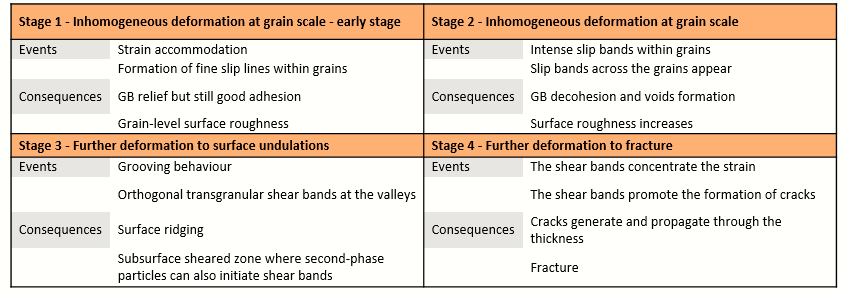
\includegraphics[width=6in]{Figures/LitRev/Stages_table_title.png}
\end{table}

\vspace{0.1 in}
\noindent
You can add Figures too, like in Figure \ref{fig:stages}, with papers cited in the caption.

\begin{figure}[H] %  figure placement: here, top, bottom, or page
    \centering
    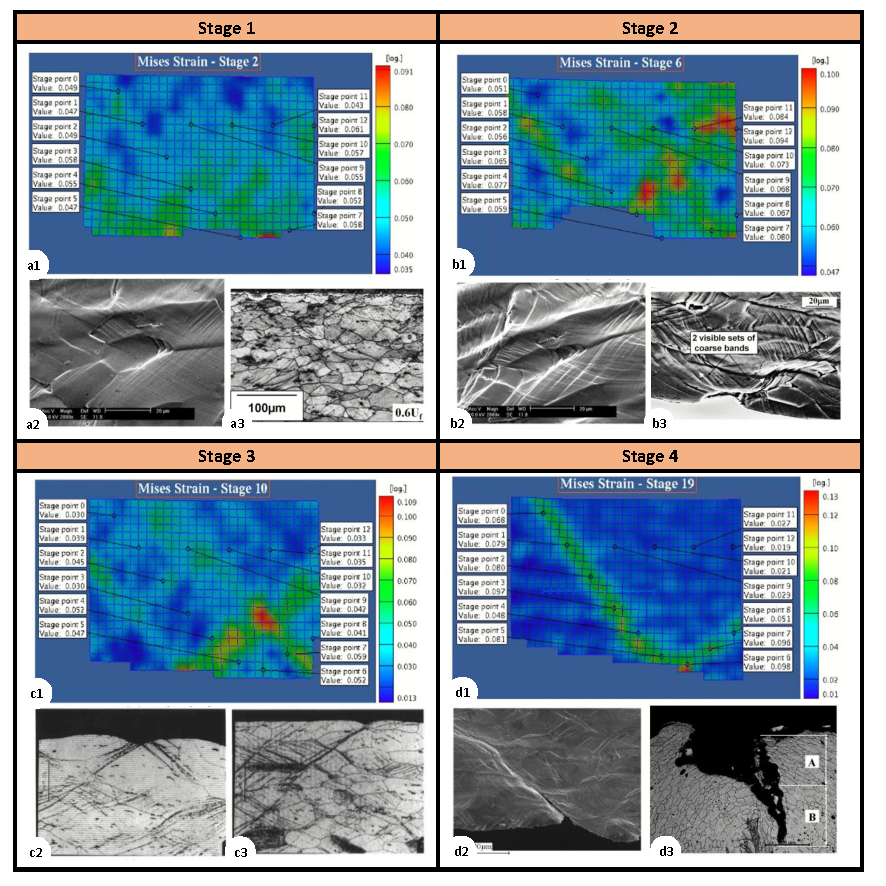
\includegraphics[width=5.5in]{Figures/LitRev/microstructural-features.pdf}
    \caption{Microstructural features at different bending stages from low (a) to high (d) degree of deformation. a1, b1, c1 and d1 are strain maps at the outer sample surface \cite{DAVIDKOV2012} (the outer surface is at the bottom of the maps). a2 \cite{DAVIDKOV2011} and a3 \cite{MATTEI2013}: thin slip lines within the grains. b2 \cite{DAVIDKOV2011} and b3 \cite{MATTEI2013}: wider slip lines and transgranular shear bands. c2 and c3: surface ridging and the subsurface sheared zone \cite{dao2001}. d2 \cite{DAVIDKOV2012} and d3 \cite{DAVIDKOV2011}: cracks that appear and propagate at the outer surface of the sample.}
    \label{fig:stages}
\end{figure}


\clearpage
\chapter{\fontsize{24pt}{20pt}\selectfont \textbf{Chapter 3}}
\section{Methodology}
\label{Chapter 3}


\clearpage
\chapter{\fontsize{24pt}{20pt}\selectfont \textbf{Chapter 4}}
\section{Chapter of results}
\label{Chapter 4}



\clearpage
\chapter{\fontsize{24pt}{20pt}\selectfont \textbf{Chapter 5}}
 \section{Second chapter of results}
\label{Chapter 5}


\clearpage
\chapter{\fontsize{24pt}{20pt}\selectfont \textbf{Chapter 6}}
 \section{A third chapter of results}
\label{Chapter 6}






\clearpage
\chapter{\fontsize{24pt}{20pt}\selectfont \textbf{Chapter 9}}
\section{Conclusions}
\label{sec:conclusions}


\clearpage
\chapter{\fontsize{24pt}{20pt}\selectfont \textbf{Chapter 10}}
\section{Future work}
\label{sec:future}


\clearpage
%\chapter{\fontsize{24pt}{20pt}\selectfont \textbf{Chapter 11}}
%\section{References}


%% If you have bibdatabase file and want bibtex to generate the
%% bibitems, please use
%%
%%
%\bibliographystyle{elsarticle-num} 
\printbibliography
%\bibliographystyle{elsarticle-num}
%\bibliography{references}
%\bibliographystyle{unsrt}
%\bibliography{references}

%% else use the following coding to input the bibitems directly in the
%% TeX file.

% \begin{thebibliography}{00}

% %% \bibitem{label}
% %% Text of bibliographic item

% \bibitem{}

% \end{thebibliography}




\end{justify}
\end{document}
\endinput

%%%%%%%%%%%%%%%%%% End of the report %%%%%%%%%%%%%%
